\documentclass[tikz,border=10pt]{standalone}
\usepackage[T1]{fontenc}
\usepackage{lmodern}
\usepackage{tikz}
\usetikzlibrary{arrows.meta,positioning,fit,shapes.geometric,backgrounds,calc}

\definecolor{datasetblue}{HTML}{D7E8F7}
\definecolor{processgreen}{HTML}{DCEED1}
\definecolor{artifactyellow}{HTML}{F7E8B2}
\definecolor{modelrose}{HTML}{F2D7D5}
\definecolor{evalgray}{HTML}{EAECEE}
\definecolor{textnavy}{HTML}{17324D}
\definecolor{lineblue}{HTML}{2C5D7C}

\tikzset{
  >={Latex[length=3mm]},
  base/.style={
    draw=lineblue,
    very thick,
    rounded corners=8pt,
    align=center,
    text=textnavy,
    minimum width=3.35cm,
    minimum height=1.25cm,
    font=\sffamily\small
  },
  dataset/.style={base, fill=datasetblue},
  process/.style={base, fill=processgreen},
  artifact/.style={base, fill=artifactyellow},
  model/.style={base, fill=modelrose},
  eval/.style={base, fill=evalgray},
  line/.style={->, very thick, draw=lineblue},
  frame/.style={
    draw=lineblue!70,
    rounded corners=10pt,
    dashed,
    inner sep=0.25cm
  }
}

\begin{document}
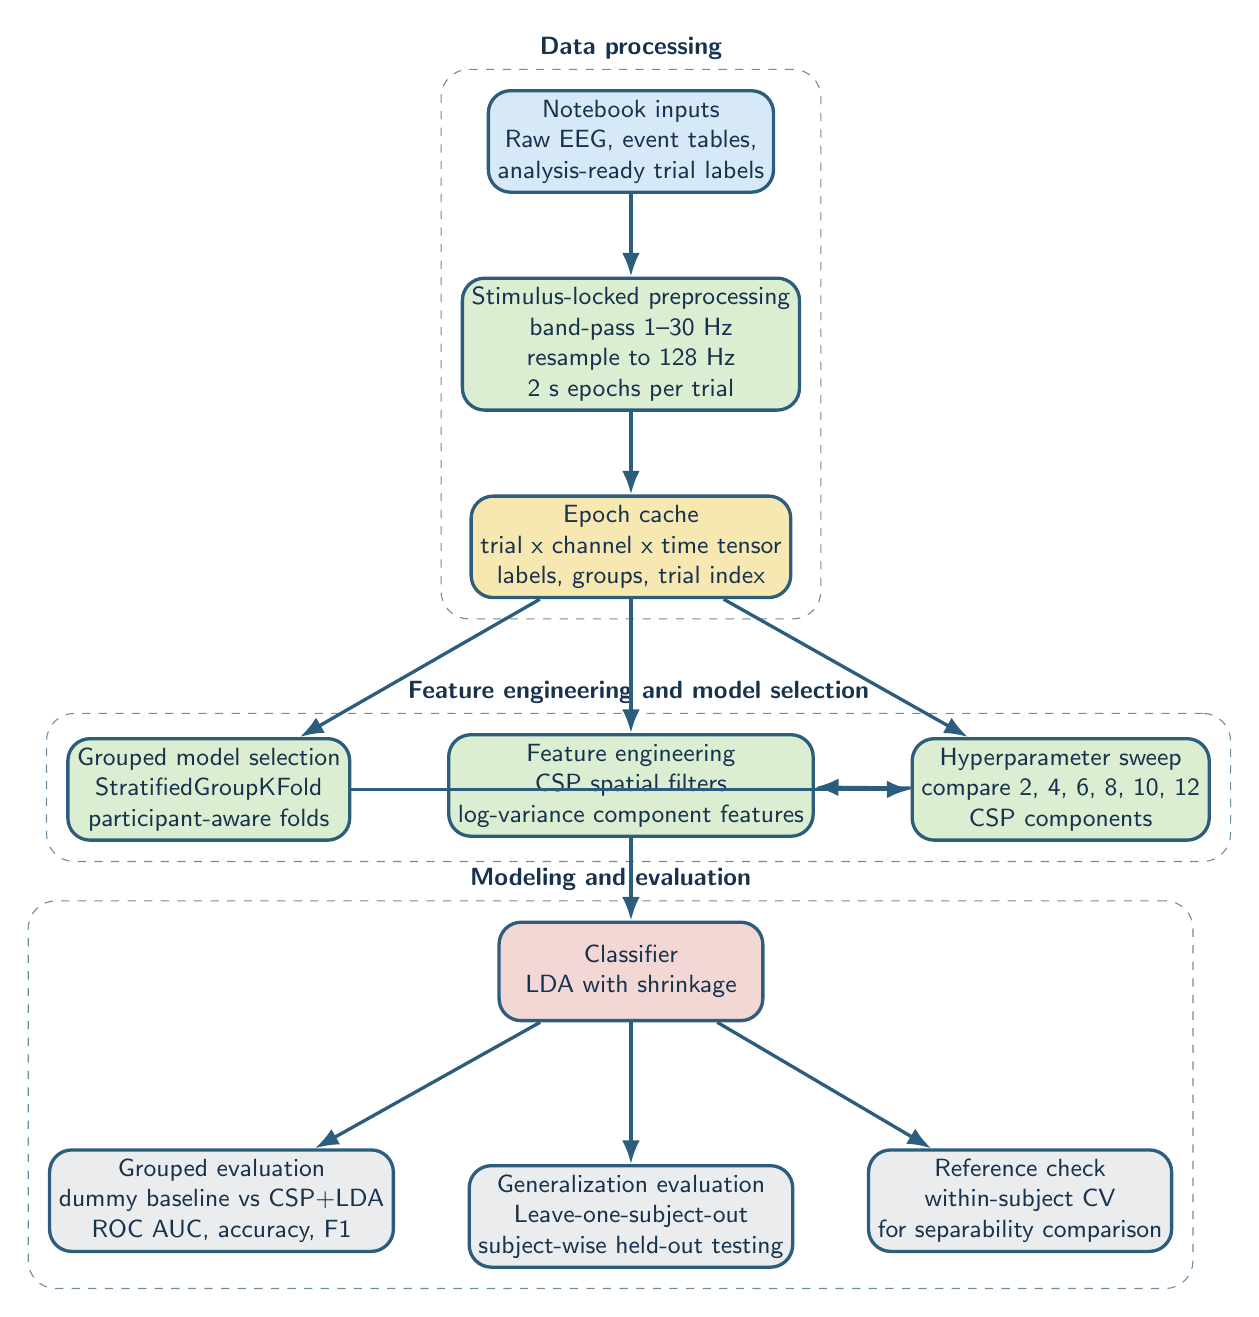
\begin{tikzpicture}[node distance=1.05cm and 1.15cm]
  \node[dataset] (raw) {Notebook inputs\\Raw EEG, event tables,\\analysis-ready trial labels};

  \node[process, below=of raw] (epoch) {Stimulus-locked preprocessing\\band-pass 1--30 Hz\\resample to 128 Hz\\2 s epochs per trial};
  \node[artifact, below=of epoch] (cache) {Epoch cache\\trial x channel x time tensor\\labels, groups, trial index};

  \node[process, below left=1.75cm and 1.5cm of cache] (groupcv) {Grouped model selection\\StratifiedGroupKFold\\participant-aware folds};
  \node[process, below=1.7cm of cache] (csp) {Feature engineering\\CSP spatial filters\\log-variance component features};
  \node[process, below right=1.75cm and 1.5cm of cache] (sweep) {Hyperparameter sweep\\compare 2, 4, 6, 8, 10, 12\\CSP components};

  \node[model, below=of csp] (lda) {Classifier\\LDA with shrinkage};
  \node[eval, below left=1.6cm and 1.3cm of lda] (groupmetrics) {Grouped evaluation\\dummy baseline vs CSP+LDA\\ROC AUC, accuracy, F1};
  \node[eval, below=1.8cm of lda] (loso) {Generalization evaluation\\Leave-one-subject-out\\subject-wise held-out testing};
  \node[eval, below right=1.6cm and 1.3cm of lda] (within) {Reference check\\within-subject CV\\for separability comparison};

  \draw[line] (raw) -- (epoch);
  \draw[line] (epoch) -- (cache);

  \draw[line] (cache) -- (csp);
  \draw[line] (cache) -- (groupcv);
  \draw[line] (cache) -- (sweep);
  \draw[line] (groupcv) -- (sweep);
  \draw[line] (sweep) -- (csp);
  \draw[line] (csp) -- (lda);
  \draw[line] (lda) -- (groupmetrics);
  \draw[line] (lda) -- (loso);
  \draw[line] (lda) -- (within);

  \begin{scope}[on background layer]
    \node[frame, fit=(raw)(epoch)(cache), label={[font=\sffamily\bfseries\small,text=textnavy]above:Data processing}] {};
    \node[frame, fit=(groupcv)(csp)(sweep), label={[font=\sffamily\bfseries\small,text=textnavy]above:Feature engineering and model selection}] {};
    \node[frame, fit=(lda)(groupmetrics)(loso)(within), label={[font=\sffamily\bfseries\small,text=textnavy]above:Modeling and evaluation}] {};
  \end{scope}
\end{tikzpicture}
\end{document}
